\chapter{ПРАКТИЧЕСКАЯ РАБОТА № 4 <<ВВЕДЕНИЕ В UML>>}

\section{Постановка задачи}

Используя открытые источники, необходимо найти и кратко описать методику использования модели «4+1» в методологии RUP, а именно указать, какой инструментарий и конкретные модели возможно использовать для отображения каждого из представления модели «4+1».

\section{Логическое или концептуальное представление}

Является объектной моделью проектирования (в том случае, если используется объектно-ориентированная модель проектирования).

Основной целью логического представления в данной методике является описание функциональных требований: что система должна выполнять в терминах конечных пользователей. Для этого представления используются различные абстрактные конструкции, такие как объекты и классы объектов. Для их иллюстрирования могут применяться диаграммы классов (в нотации языка UML) либо, например, диаграммы <<сущность-связь>>, если в разработке приложения доминируют данные.

Для этого представления подойдет диаграмма Прецедентов (RUP).

Унифицированный процесс --- это процесс, управляемый прецедентами, которые отражают сценарии взаимодействия пользователей. Фактически, это взгляд пользователей на программную систему снаружи. Таким образом, одним из важнейших этапов разработки, согласно RUP, будет этап определения требований, который заключается в сборе всех возможных пожеланий к работе системы, которые только могут прийти в голову пользователям и аналитикам. Позднее эти данные должны будут систематизированы и структурированы, но на данном этапе в ходе интервью с пользователями и изучения документов, аналитики должны собрать как можно больше требований к будущей системе, что не так просто, как кажется на первый взгляд. Пользователи часто сами не представляют, что они должны получить в конечном итоге. Для облегчения этого процесса аналитики используют диаграммы прецедентов.

Диаграмма представляет собой отражение действующих лиц (актантов), которые взаимодействуют с системой, и реакцию программных объектов на их действия. Актантами могут быть как пользователи, так и внешние агенты, которым необходимо передать или получить информацию. Значок варианта использования отражает реакцию системы на внешнее воздействие и показывает, что должно быть сделано для актанта.

Простота диаграммы прецедентов позволяет аналитикам легко общаться с заказчиками в процессе определения требований, выявлять ограничения, налагаемые на систему и на выполнение отдельных требований, такие, например, как время реакции системы, которые в дальнейшем попадают в раздел нефункциональных требований.

\begin{figure}[h!]
        \centering
        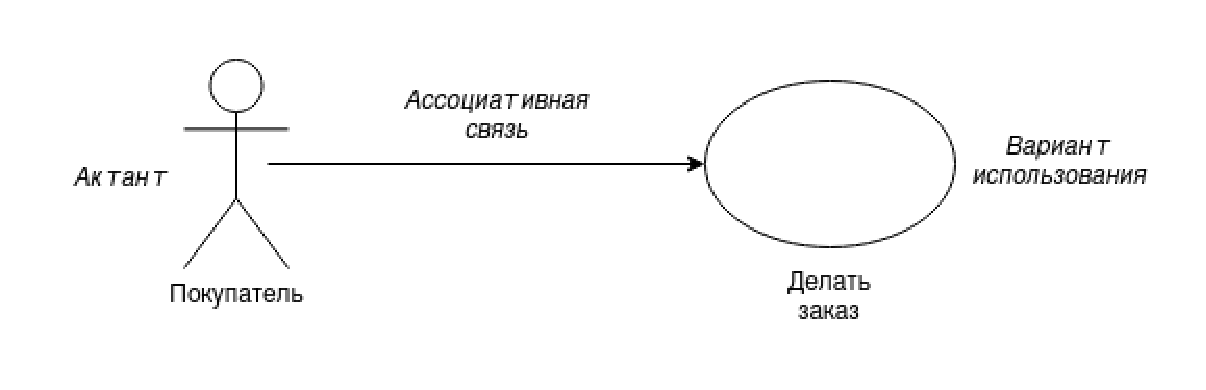
\includegraphics[width=\textwidth]{images/4/1.eps}
        \caption{Диаграмма прецедентов}
\end{figure}

\section{Представление процесса}

Описывает вопросы параллельного исполнения и синхронизации процессов.

Процессное представление учитывает некоторые нефункциональные требования к системе, включая производительность и доступность. С помощью этого представления рассматриваются такие аспекты, как одновременное выполнение и распределение процессов, интеграция системы, устойчивость к сбоям, а также то, как основные объекты абстракции, рассмотренные на уровне логического представления, соответствуют архитектуре процессов. Архитектура процессов может быть представлена на различных уровнях абстракции. На самом высоком уровне система рассматривается как набор независимо выполняемых сетей взаимодействующих между собой программ. На более низких уровнях рассматриваются процессы и задачи.

Для этого представления подойдет диаграмма Активности (RUP).

\begin{figure}[h!]
        \centering
        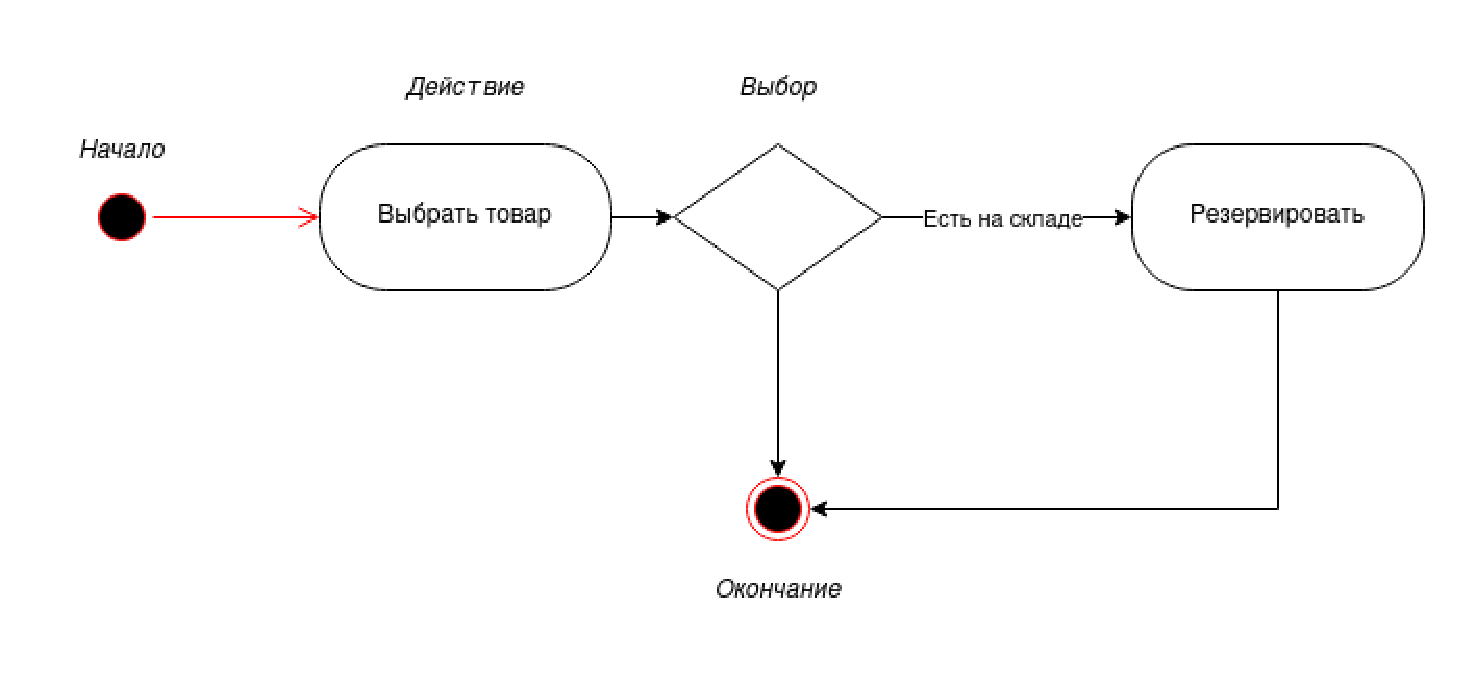
\includegraphics[width=\textwidth]{images/4/2.eps}
        \caption{Диаграмма Активности}
\end{figure}

\section{Физическое представление}
Описывает размещение программных компонент системы на аппаратных платформах и аспекты, связанные с физическим расположением системы.

Физическое представление, в основном, рассматривает нефункциональные требования, такие как доступность, надежность, устойчивость, производительность, масштабируемость. Этот уровень описывает распределение различных элементов --- сетей, процессов, задач и объектов --- по различным узлам (элементам аппаратного обеспечения, объединенным в сеть).

Для этого представления подходит реализация (RUP).

Основная задача процесса реализации – создание системы в виде компонентов – исходных текстов программ, сценариев, двоичных файлов, исполняемых модулей и т.д. На этом этапе создается модель реализации, которая описывает то, как реализуются элементы модели проектирования, какие классы будут включены в конкретные компоненты. Данная модель описывает способ организации этих компонентов в соответствии с механизмами структурирования и разбиения на модули, принятыми в выбранной среде программирования и представляется диаграммой компонентов.

\begin{figure}[h!]
        \centering
        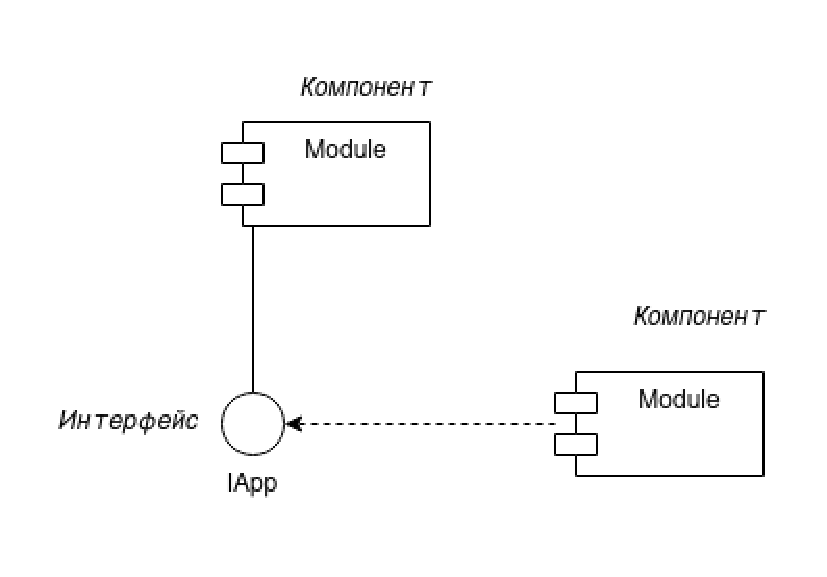
\includegraphics[width=0.6\textwidth]{images/4/3.eps}
        \caption{Диаграмма реализации}
\end{figure}

\section{Представление уровня разработки}

Описывает статическую организацию программной системы в среде разработки.

Представление уровня разработки описывает фактическую организацию модулей системы, разделение ее на подсистемы, которые могут разрабатываться независимо.

Для этого представления подходит тестирование (RUP).

В процессе тестирования проверяются результаты реализации. Для данного процесса создается модель тестирования, которая состоит из тестовых примеров, процедур тестирования, тестовых компонентов, однако не имеет отображения на UML диаграммы.

\section{Вывод}

Используя открытые источники, нашли и кратко описали методику использования модели «4+1» в методологии RUP, указали, какой инструментарий и конкретные модели возможно использовать для отображения каждого из представления модели «4+1».

